% Relatório do laboratório 3 de servo
% Felipe Bandeira da Silva
% 09/06/2013

%\documentclass[a4paper, 10pt]{article}
\documentclass[paper=a4, fontsize=11pt]{article}

\usepackage[framed,numbered,autolinebreaks,useliterate]{mcode}

\usepackage[brazil]{babel}
\usepackage[utf8]{inputenc}
\usepackage{listings}
\usepackage{color}
\usepackage{amsthm}
\usepackage{graphicx}

\setlength{\parindent}{0pt}
\setlength{\parskip}{18pt}

\title{Relatório, Laboratório 4.\\Servo 1}
\author{Felipe Bandeira da Silva}


%%%%%%%%%%%%%%%%%%%%%%%%%%%%%%%%%%%%%%%%%%%%%%%%%%%%%%%%%%%%%%%%%%%%%%%%%%%%%%%%
% MAIN
%%%%%%%%%%%%%%%%%%%%%%%%%%%%%%%%%%%%%%%%%%%%%%%%%%%%%%%%%%%%%%%%%%%%%%%%%%%%%%%%

\begin{document}

\maketitle

\begin{abstract}
Utilizar o Matlab para analisar a resposta transitória de sistemas de 1ª ordem
ao degrau e estudar o efeito do controle proporcional sobre os aspectos de
estabilidade, velocidade de resposta e erro em regime permanente.
\end{abstract}


\newpage

%%%%%%%%%%%%%%%%%%%%%%%%%%%%%%%%%%%%%%%%%%%%%%%%%%%%%%%%%%%%%%%%%%%%%%%%%%%%%%%
% QUESTÃO 1
%%%%%%%%%%%%%%%%%%%%%%%%%%%%%%%%%%%%%%%%%%%%%%%%%%%%%%%%%%%%%%%%%%%%%%%%%%%%%%%
\section{Primeira questão}

O primeiro sistema fisico é modelado com a equação 1
\begin{equation}
    G_1(s) = \frac{1}{s+1}
\end{equation}

A equação temporal da equação 1 quando submetida a um degrau unitário
é facilmente encontrada aplicando a transformada inversa de laplace,

\begin{equation}
    G_1(s) = \frac{1}{s+1} \frac{1}{s}
\end{equation}

Aplicando o comando $residue$ em 2 para a expansão em frações parciais,

\begin{equation}
    G_1(s) = \frac{-1}{s+1} + \frac{1}{s}
\end{equation}

De 3 é possível encontrar a reposta temporal,

\begin{equation}
    g_1(t) = -e^{-t} + 1
\end{equation}

A plotagem do gráfico pode ser usada para a facilitar o visualização
do comportamento da função,

\begin{center}
    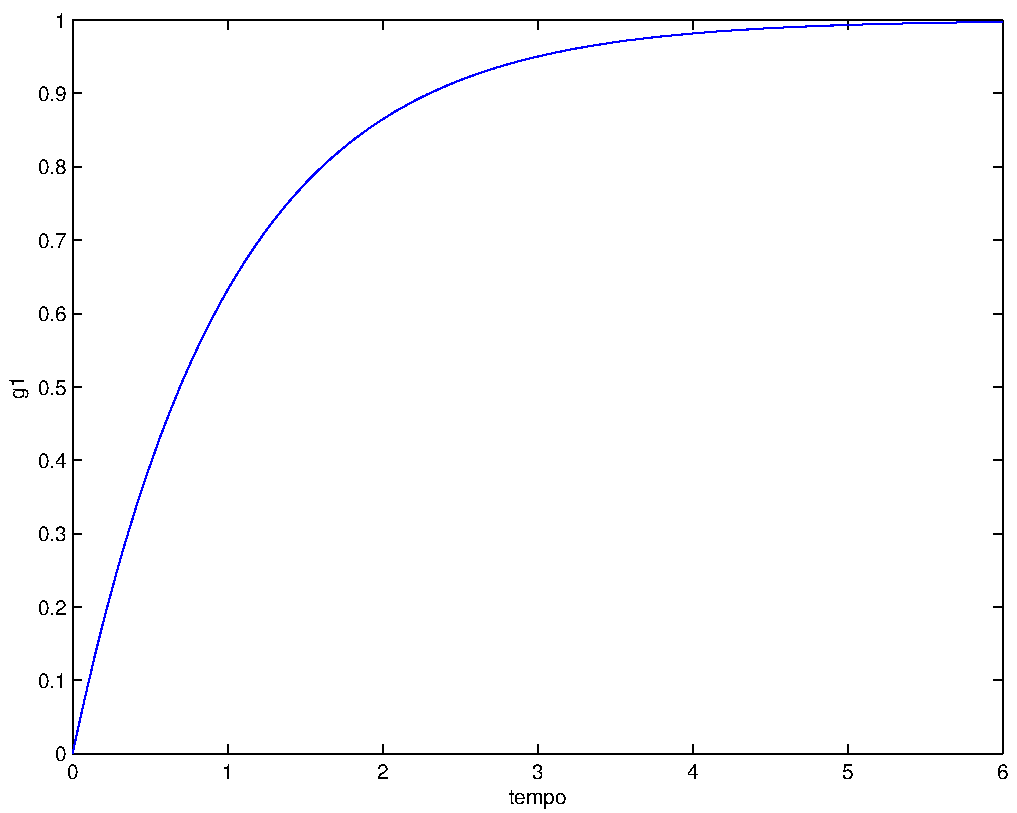
\includegraphics[scale=.5]{q1g1.pdf}
\end{center}

Por inspeção é possível notar que o sistema se estabiliza após um tempo
e seu valor em regimente permanente é 1. Mostrando que o sistema apresenta
uma estabilidade. Esta estabilidade pode ser melhor analisada plotando
a localização dos polos no plano-s.

\begin{center}
    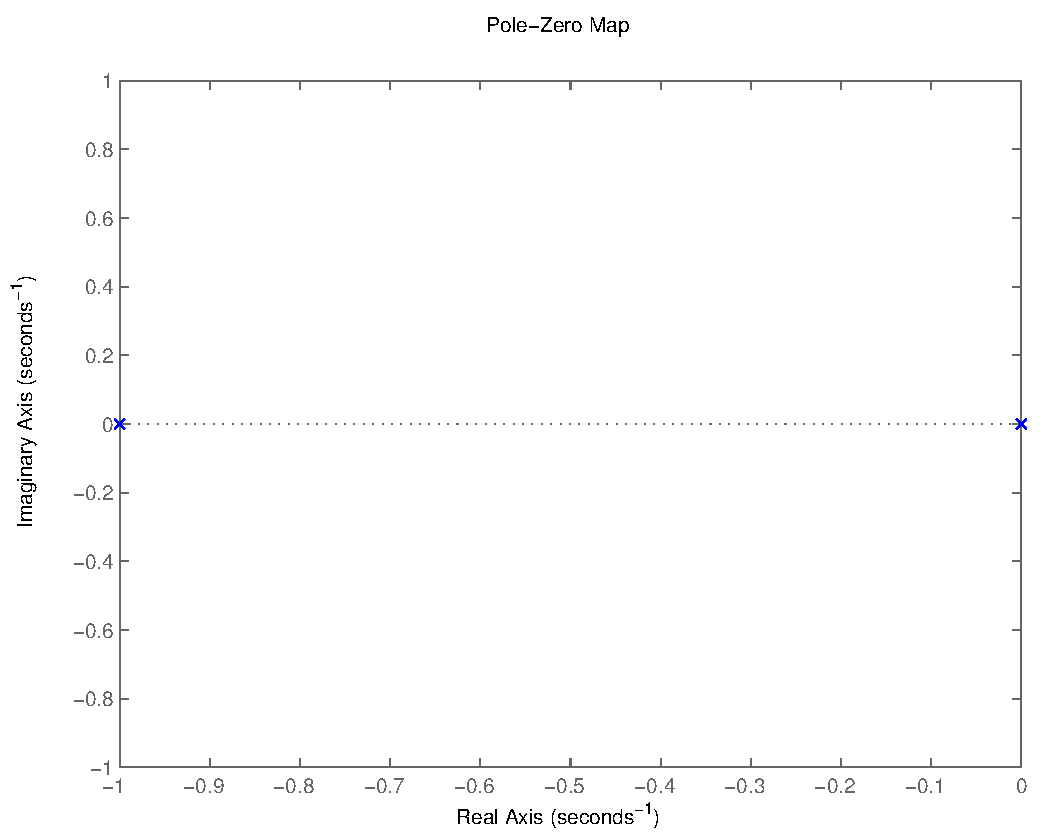
\includegraphics[scale=.5]{pzq1g1.pdf}
\end{center}

Como é possível observar existem dois polos no eixo real e com valores 
menor igual a zero, mostrando que o sistema é \textbf{estável}. Fato este
que está diretamente ligado a posição dos polos no eixo $\sigma$(eixo real).

Analisando agora a funçao,

\begin{equation}
    G_2(s) = \frac{1}{s-1}
\end{equation}

Expandindo em frações parciais,

\begin{equation}
    G_2(s) = \frac{1}{s+1} + \frac{-1}{s}
\end{equation}

A função no domínio do tempo com resposta ao impulso unitário é,

\begin{equation}
    g_2(t) =  e^{t} - 1
\end{equation}

A função 5 será analisada da mesma forma que a 1, só que usando comandos
mais poderosos do matlab, para tanto, uso o comando $tf$ para construir 
a função de transferência, após isto uso o comando $step$ para a criação
dos vetores com os eixos do domínio e imagem, finalmente obtenho o grafico
da resposta temporal,

\begin{center}
    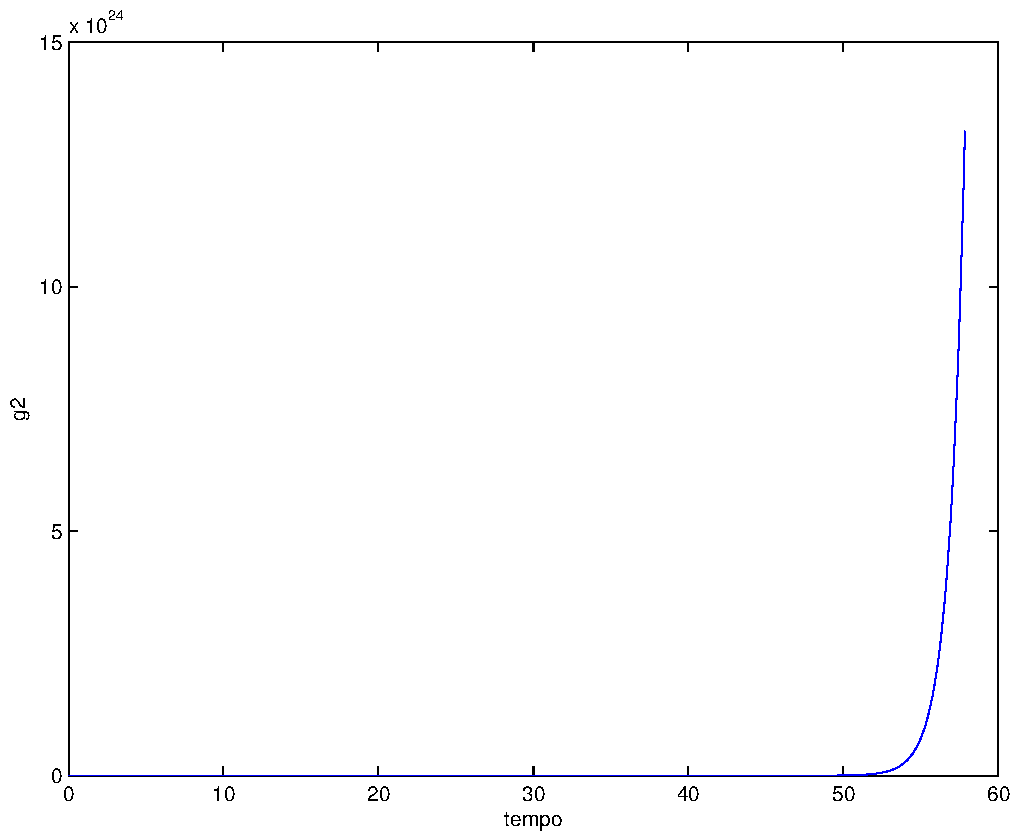
\includegraphics[scale=.5]{q1g2.pdf}
\end{center}

Nota-se que o valor de $g2$ cresce de forma exponencial e tente ao infinito, 
novamente por inspeção é possível concluir que o sistema é instável. Para
formalizar a conclusão, a figura abaixo mostra o plano-s,

\begin{center}
    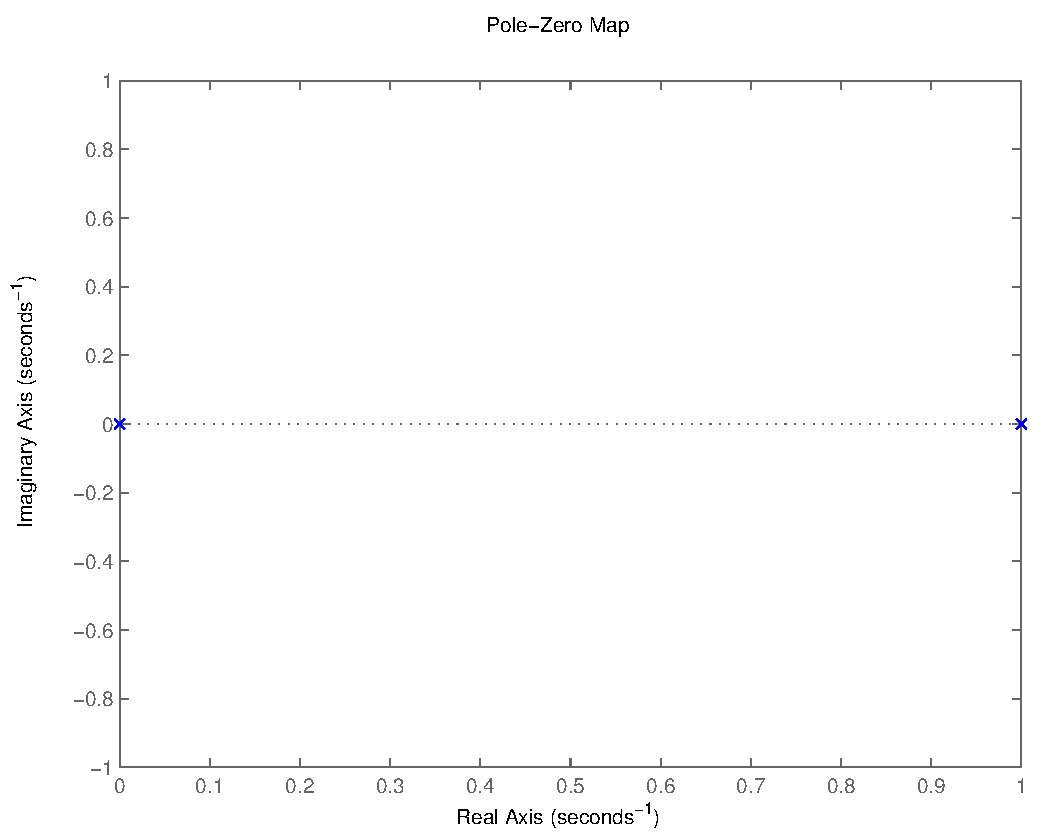
\includegraphics[scale=.5]{pzq1g2.pdf}
\end{center}

Nota-se que os polos são positivos e portanto na zona de instabilidade do plano-s.

Sobrepondo os dois gráficos da resposta temporal,

\begin{center}
    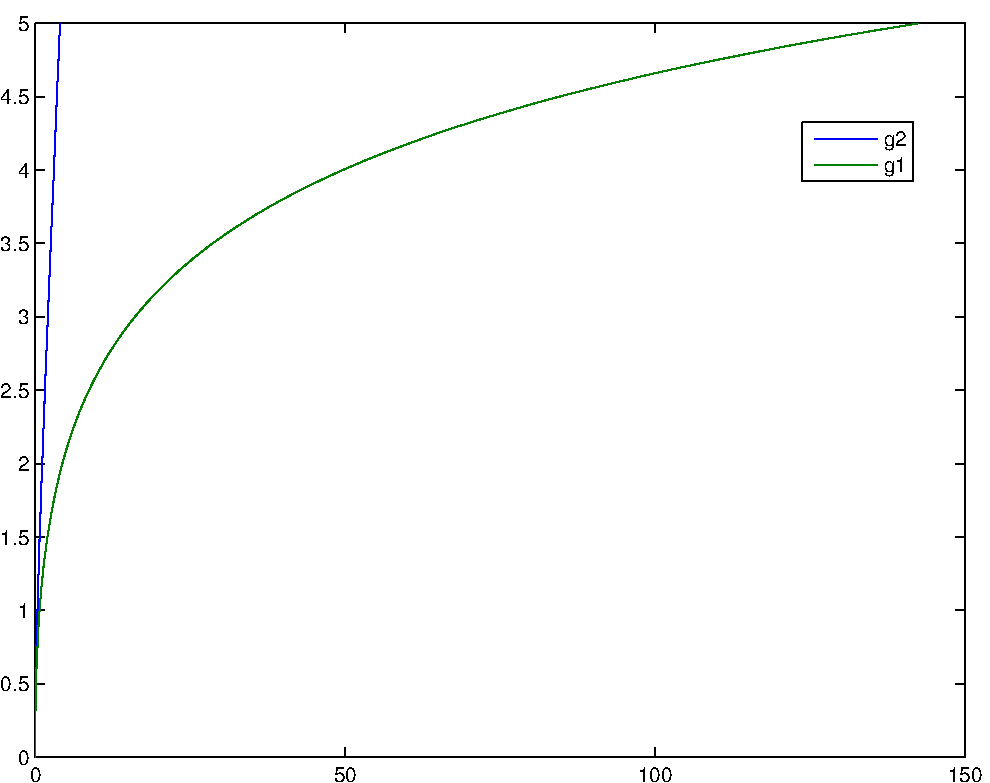
\includegraphics[scale=.5]{g1g2.pdf}
\end{center}

É possível visualizar que a função $g2$ cresce "infinitamente" mais rápida que $g1$
Finalmente é possível ver que a posição dos polos influencia facilmente a 
estabilidade de um sistema, é que o plano-s é uma ótima forma que visualizar
esta tal estabilidade, se contraponto até mesmo ao gráfico da resposta temporal.

%%%%%%%%%%%%%%%%%%%%%%%%%%%%%%%%%%%%%%%%%%%%%%%%%%%%%%%%%%%%%%%%%%%%%%%%%%%%%%%%
% SEGUNDA QUESTÃO
%%%%%%%%%%%%%%%%%%%%%%%%%%%%%%%%%%%%%%%%%%%%%%%%%%%%%%%%%%%%%%%%%%%%%%%%%%%%%%%%

\section{Segunda questão}

Para este problema foram propostos os seguintes sistemas,

\begin{center}
    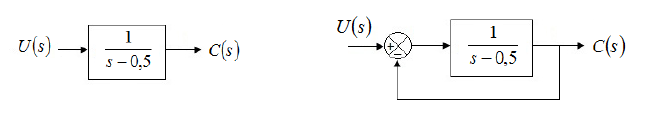
\includegraphics[scale=.5]{s2q.png}
\end{center}

Caracterizando cada sistema, tenho para o primeiro(lado esquerdo), a posição 
dos polos,

\begin{center}
    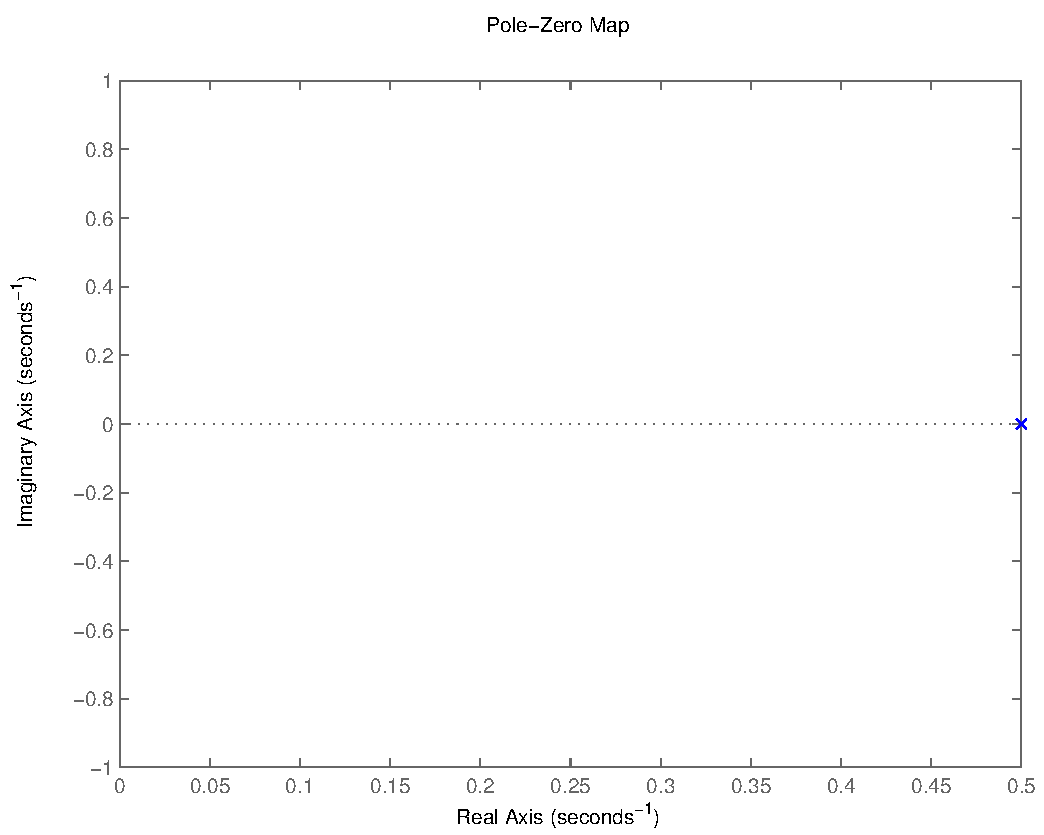
\includegraphics[scale=.5]{pz2qs1.pdf}
\end{center}




\end{document}
